\chapter*{Conclusione}
\addcontentsline{toc}{chapter}{Conclusione}
L'obiettivo di questa tesi era mostrare a che livello e in che misura
il requisito della scalabilità e l'utilizzo delle risorse in cloud impattano sulla realizzazione di un'applicazione.\\
\\
Durante la fase di analisi è stato evidenziato quali fossero i punti critici del progetto.
Si sono quindi affiancate a ogni componente scelto le necessità a cui dovevano rispondere,
eventualmente approfondendo le molteplici offerte presenti sul mercato.
La scelta è stata determinata dalle tecnologie e funzionalità che presentavano, 
influenzando in maniera decisiva l'approccio da usare
nella progettazione del codice.
Sono state quindi affiancate le scelte implementative implicate dall'utilizzo dei vari servizi.\\
\begin{figure}[htbp]
    \begin{center}
        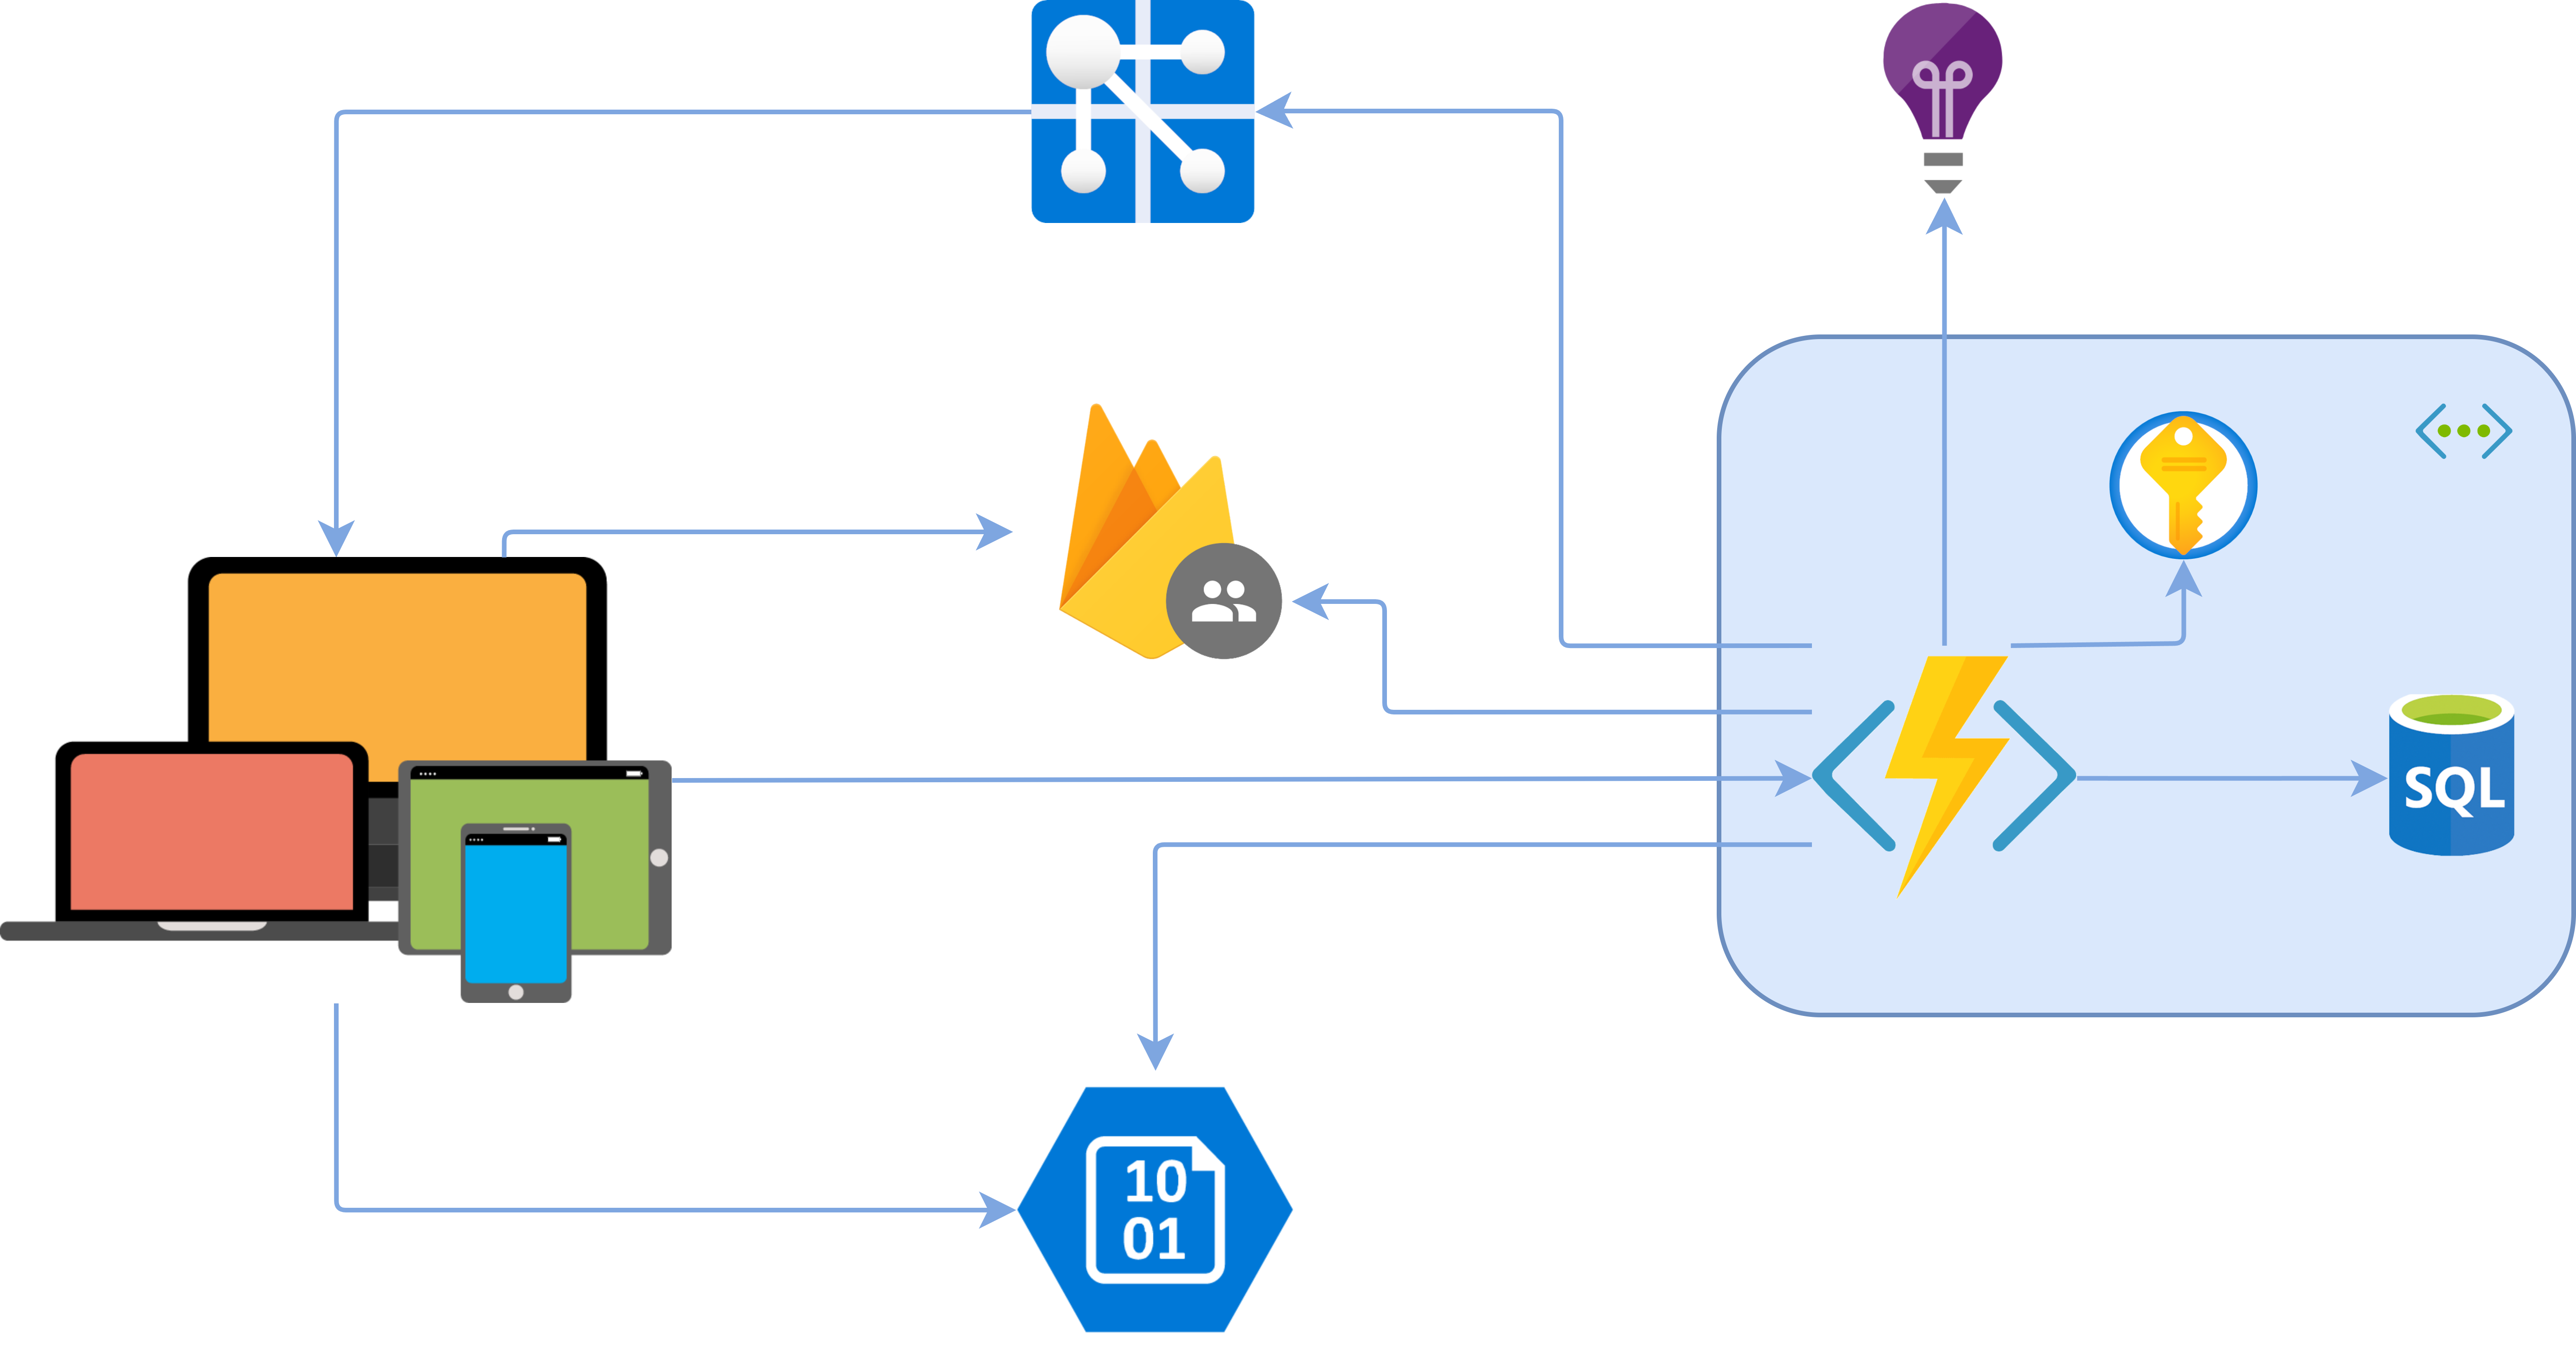
\includegraphics[width=\textwidth]{ImplementazioneArchitettura.png}
        \caption{Grafico dell'architettura di WYD}
    \end{center}
\end{figure}
\clearpage
La fase di realizzazione ha visto lo sviluppo di un client utente intuitivo 
e di un server scalabile ed efficiente, sfruttando la tecnologia serverless.
Una particolare attenzione è stata prestata ai meccanismi di autenticazione, 
alla sicurezza dei dati e al monitoraggio continuo dei servizi.
La gestione della persistenza è stata affrontata 
attraverso l'implementazione di un database non relazionale distribuito,
scelta che ha comportato il principale impatto sulle dinamiche del progetto.
Gli è stato inoltre affiancato lo sviluppo 
di una memoria locale per la cache e la comunicazione in tempo reale, 
elementi cruciali per la reattività dell'applicativo.
Un capitolo significativo è stato dedicato al recupero e al salvataggio dei dati multimediali, 
essenziali per la funzionalità di condivisione in tempo reale di Wyd.\\
\\
L'integrazione tra le tecnologie cloud ha richiesto 
un approccio progettuale orientato alla separazione delle responsabilità, 
alla gestione della consistenza eventuale e alla resilienza in caso di errori o richieste concorrenti. Ciò ha condotto all'adozione di pattern moderni, 
come la denormalizzazione, i trigger su modifiche, 
l'uso di code per la propagazione degli eventi e 
notifiche in tempo reale attraverso canali dedicati.\\
\\
I risultati ottenuti durante i test di carico hanno confermato 
la qualità delle scelte architetturali adottate: 
il sistema dimostra di sostenere centinaia di richieste al secondo 
senza degrado percettibile delle prestazioni, 
mantenendo al tempo stesso un basso tempo di latenza.\\
\\
In definitiva, il percorso intrapreso ha mostrato 
come la realizzazione di un'applicazione distribuita e scalabile 
non sia il frutto di un processo lineare, 
ma di un dialogo costante tra le esigenze funzionali, 
i vincoli tecnologici e le opportunità offerte dai servizi cloud-native. 
Ogni tecnologia adottata ha influito sulle logiche implementative, 
imponendo precise scelte progettuali, 
sia in termini di prestazioni che di costi.\\
\\
L'auspicio è che le considerazioni sviluppate 
possano offrire un contributo utile non solo alla valutazione di Wyd come progetto,
ma anche come punto di partenza per l'approfondimento dei principi e delle pratiche 
legate allo sviluppo di applicazioni moderne, condivise e scalabili.
\clearpage

\section{Sviluppi futuri}

Wyd può essere ampliata nelle sue funzionalità,
con conseguenze sull'infrastruttura che possono essere nulle o molto impattanti.\\
\\
L'architettura attuale guadagnerebbe sicuramente in prestazioni dall'introduzione
di una cache tra le Azure Functions e il database.
È inoltre bene rivedere l'utilizzo delle websocket per le informazioni in tempo reale, 
considerato l'impatto previsto di Azure PubSub sui costi totali.\\
\\
L'implementazione di eventi pubblici è sicuramente il principale passo logico successivo 
per rendere Wyd un'applicazione di ampio utilizzo.
Questo comporta la realizzazione di una piattaforma dedicata,
che riceva gli eventi e ne gestisca la condivisione,
tenendo traccia di tutti i rapporti tra profili che seguono e 
profili che possono pubblicare.\\
\\
Con la creazione di eventi pubblici ha senso prevedere un sistema 
per gestire la prenotazione e l'organizzazione degli eventi,
dalle liste di attesa alle vendite dei biglietti.
La necessità di garantire la robustezza del servizio,
introducendo logiche di controllo dei ruoli e di traffico monetario,
comporta requisiti specifici di affidabilità e consistenza 
a cui l'infrastruttura dovrà rispondere.\\
\\
Vista la crescente attenzione alla privacy, 
alla protezione dei dati e alla dipendenza dovuta all'utilizzo di servizi esterni,
si prevede di sviluppare un applicativo gemello 
che possa essere distribuito su un unico server dedicato,
per fornire la possibilità a terzi di eseguire su macchine proprie.
Il programma vedrebbe quindi un'infrastruttura fisica completamente diversa,
ma la sua implementazione continuerebbe a seguire
tutti i principi adottati per mantenere il codice scalabile,
fornendo così un prodotto comunque resistente a carichi differenti, seppure ridotti.
Questo diminuirebbe inoltre il numero di modifiche da introdurre nel codice.\\
\\
Infine, ulteriori sviluppi potranno comprendere, in base alle necessità degli utenti:
\begin{itemize}
    \item La visualizzazione degli impegni degli altri profili
    \item L'implementazione di una chat per ogni gruppo
    \item Strumenti utili all'organizzazione dei gruppi, quali:
          \begin{itemize}
              \item form per combinare le disponibilità reciproche
              \item appunti condivisi(liste della spesa o note su chi porta cosa)
              \item calcolo delle spese compiute da ciascun componente
          \end{itemize}
    \item Una funzionalità di ricerca degli eventi o dei profili pubblici
\end{itemize}
\clearpage